\documentclass[12pt]{article}

\usepackage[english]{babel}
\usepackage[utf8]{inputenc}
\usepackage{fancyhdr}

\usepackage[margin=1in]{geometry}
\usepackage{pgf}
\usepackage{pgfplots}
\usepackage{siunitx}
\usepackage{tikz}
\usepackage{float}
\usepackage{amsmath}
\usepackage{enumitem}
\usepackage{textcomp}
\usepackage{hyperref}

\usepackage[font=small,labelfont=bf]{caption}
\usepackage[nodisplayskipstretch]{setspace}

\usetikzlibrary{scopes}
\usetikzlibrary{angles,quotes}
\usetikzlibrary{calc}
\graphicspath{ {/} }
\pgfplotsset{compat=1.5}

\newcommand*{\I}{\imath}
\newcommand*{\J}{\jmath}
\newcommand{\norm}[1]{\lvert #1 \rvert}

\setlist[enumerate, 1]{label=\alph*.}

\begin{document}
\sisetup{per-mode=symbol}

\begin{titlepage}
    \begin{center}
        \vspace*{1cm}
        \textbf{Electric Circuits 2}

        \vspace{0.5cm}
        Lab: 02

        \vspace{1cm}

        \textbf{Jaden Moore}

        \vfill

        Orange Coast College\\
        Engineering Circuits A285\\
        December 7th, 2021

    \end{center}
\end{titlepage}

\pagestyle{fancy}
\fancyhf{}
\setlength{\headheight}{15pt}
\lhead{Electric Circuits 2}
\rhead{Lab: 02}
\cfoot{\thepage}

\section{Introduction}
In this lab, we attach a resistance $R_L$ across two end terminals of a circuit. We then analyze the behavior of the various electrical quantities across the resistor as the resistance increases. We then prove Thévenin's theorem by creating Thévenin's equivalent circuit and comparing the electrical quantities with the original circuit quantities. Throughout the lab, we utilize the web based circuit builder CircuitLab to generate and analyze the circuit.

\begin{figure}[H]
    \begin{center}
        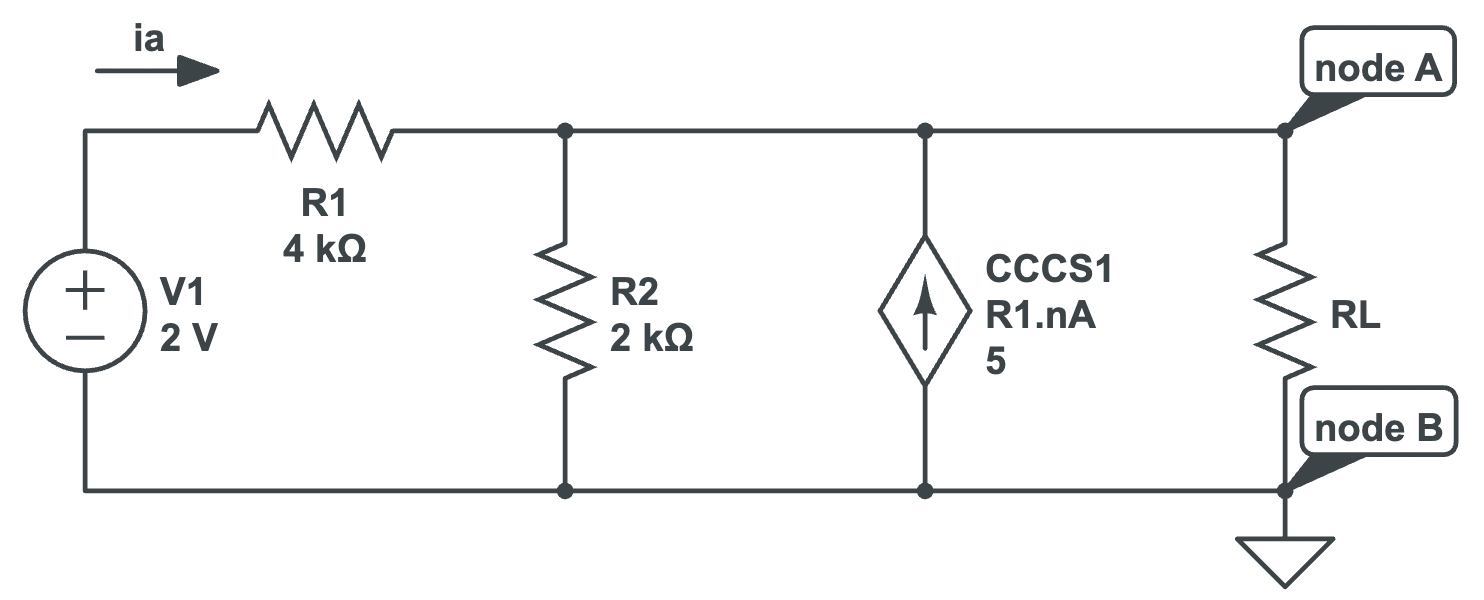
\includegraphics[scale=0.6]{circuit-1.png}
        \caption { Electric circuit with resistor $R_L$ across terminals A-B}
    \end{center}
\end{figure}
Consider the circuit presented in Figure (1). We place increasing resistances across $R_L$ and measure the current $i_L$, the voltage, $v_L$, and power $p_L$ across the resistor and record the data in the table below.
\section{Data}
\newcolumntype{P}[1]{>{\arraybackslash}p{#1}}

\setlength{\tabcolsep}{2pt}
\renewcommand{\arraystretch}{1.1}

\begin{figure}[H]
    \begin{center}
        \begin{tabular}{ P{2.5cm}|P{2.5cm} P{2.5cm} P{2.5cm} P{2.5cm} }
            \hline
            \multicolumn{5}{c}{Table 1: Data collected from CircuitLab for different resistances $R_L$} \\

            \hline
            $R_L$ [$\Omega$] & $i_L$ [A] & $v_L$ [V]  & $p_{L}$	[W] & $p_{L-theory}$ [W] \\
            \hline
            10               & 2.941E-03 & 029.41E-03 & 086.5E-06  & 086.505E-06        \\
            56               & 2.698E-03 & 151.08E-03 & 407.6E-06  & 407.588E-06        \\
            110              & 2.459E-03 & 270.49E-03 & 665.1E-06  & 665.144E-06        \\
            180              & 2.206E-03 & 397.06E-03 & 875.9E-06  & 875.865E-06        \\
            200              & 2.143E-03 & 428.57E-03 & 918.4E-06  & 918.367E-06        \\
            270              & 1.948E-03 & 525.97E-03 & 1.025E-03  & 001.025E-03        \\
            360              & 1.744E-03 & 627.91E-03 & 1.095E-03  & 001.095E-03        \\
            430              & 1.613E-03 & 693.55E-03 & 1.119E-03  & 001.119E-03        \\
            470              & 1.546E-03 & 726.80E-03 & 1.124E-03  & 001.124E-03        \\
            560              & 1.415E-03 & 792.45E-03 & 1.121E-03  & 001.121E-03        \\
            750              & 1.200E-03 & 900.00E-03 & 1.080E-03  & 001.080E-03        \\
            1000             & 1.000E-03 & 1.000      & 1.000E-03  & 001.000E-03        \\
            1800             & 652.2E-06 & 1.174      & 765.6E-06  & 765.595E-06        \\
            2700             & 468.8E-06 & 1.266      & 593.3E-06  & 593.262E-06        \\
            3600             & 365.9E-06 & 1.317      & 481.9E-06  & 481.856E-06        \\
            5600             & 245.9E-06 & 1.377      & 338.6E-06  & 338.619E-06        \\
            27000            & 54.55E-06 & 1.473      & 80.33E-06  & 080.331E-06        \\
            110000           & 13.57E-06 & 1.493      & 20.27E-06  & 020.270E-06        \\
            220000           & 6.803E-06 & 1.497      & 10.18E-06  & 010.181E-06        \\
            750000           & 1.999E-06 & 1.499      & 2.996E-06  & 002.996E-06        \\
            1100000          & 1.363E-06 & 1.499      & 2.044E-06  & 002.044E-06        \\
            2400000          & 624.9E-09 & 1.500      & 937.1E-09  & 937.109E-09        \\
            4700000          & 319.1E-09 & 1.500      & 478.6E-09  & 478.622E-09        \\
            6200000          & 241.9E-09 & 1.500      & 362.8E-09  & 362.845E-09        \\
            8200000          & 182.9E-09 & 1.500      & 274.4E-09  & 274.357E-09        \\
            10000000         & 150.0E-09 & 1.500      & 225.0E-09  & 224.978E-09        \\

            \hline
        \end{tabular}
    \end{center}
\end{figure}
Using the table above, we plot the electrical quantities over the resistance $R_L$ to further identify and analyze the trends.
\begin{figure}[H]
    \centering
    \begin{tikzpicture}
        \pgfplotsset{width=10cm}
        \begin{axis}[
                xlabel={$R_L$ [$\Omega$]},
                ylabel={$i_L$ [A]},
                xmode=log,
                scaled y ticks=false,
                legend cell align = left,
                legend pos = north east,
                xtick pos=left,
                ytick pos=left
            ]
            \addplot[red, only marks, mark=o, smooth,tension={0.5}] table{CvR.txt};

            \addlegendimage{only marks}
            \addlegendentry{current $i_L$}
        \end{axis}
    \end{tikzpicture}
    \caption[12pt]{Current through load resistance $R_L$}
\end{figure}

\begin{figure}[H]
    \centering
    \begin{tikzpicture}
        \pgfplotsset{width=10cm}
        \begin{axis}[
                xlabel={$R_L$ [$\Omega$]},
                ylabel={$v_L$ [V]},
                xmode=log,
                scaled y ticks=false,
                legend cell align = left,
                legend pos = south east,
                xtick pos=left,
                ytick pos=left
            ]
            \addplot[blue, only marks, mark=o, smooth,tension={0.5}] table{VvR.txt};

            \addlegendimage{only marks}
            \addlegendentry{voltage $v_L$}
        \end{axis}
    \end{tikzpicture}
    \caption[12pt]{Voltage through load resistance $R_L$}
\end{figure}

\begin{figure}[H]
    \centering
    \begin{tikzpicture}
        \pgfplotsset{width=10cm,compat=1.3}
        \begin{axis}[
                xlabel={$R_L$ [$\Omega$]},
                ylabel={$i_L$ [A]},
                axis y line*=left,
                xmode=log,
                scaled ticks=false,
            ]
            \addplot[red, only marks, mark=o, smooth,tension={0.5}] table{CvR.txt}; \label{plot_1}
        \end{axis}

        \begin{axis}[
                xlabel={$R_L$ [$\Omega$]},
                ylabel={$v_L$ [V]},
                xmode=log,
                scaled y ticks=false,
                hide x axis,
                axis y line*=right,
                legend cell align = left,
                legend style={at={(0.95,0.6)},anchor=north east}
            ]
            \addplot[blue, only marks, mark=o, smooth,tension={0.5}] table{VvR.txt}; \label{plot_2}

            \addlegendimage{/pgfplots/refstyle=plot_1}\addlegendentry{voltage $v_L$}
            \addlegendimage{/pgfplots/refstyle=plot_2}\addlegendentry{current $i_L$}
        \end{axis}

    \end{tikzpicture}
    \caption[12pt]{Current and voltage through load resistance $R_L$}
\end{figure}

\begin{figure}[H]
    \centering
    \begin{tikzpicture}
        \pgfplotsset{width=10cm}
        \begin{axis}[
                xlabel={$R_L$ [$\Omega$]},
                ylabel={$p_L$ [W]},
                xmode=log,
                scaled y ticks=false,
                legend cell align = left,
                legend pos = north east,
                xtick pos=left,
                ytick pos=left
            ]
            \addplot[orange, only marks, mark=o, smooth,tension={0.5}] table{PvR.txt};

            \addlegendimage{only marks}
            \addlegendentry{power $p_L$}
        \end{axis}
    \end{tikzpicture}
    \caption[12pt]{Power $p_L$ through load resistance $R_L$}
\end{figure}

\begin{figure}[H]
    \centering
    \begin{tikzpicture}
        \pgfplotsset{width=10cm}
        \begin{axis}[
                xlabel={$R_L$ [$\Omega$]},
                ylabel={$i_a$ [A]},
                xmode=log,
                ymax=0.0009,
                ymin=0.00000001,
                scaled y ticks=false,
                legend cell align = left,
                legend pos = north east,
                xtick pos=left,
                ytick pos=left
            ]
            \addplot[teal, only marks, mark=o, smooth] table{CSvR.txt};

            \addlegendimage{only marks}
            \addlegendentry{current $i_a$}
        \end{axis}
    \end{tikzpicture}
    \caption[12pt]{Current $i_a$ through voltage source $v_1$ over resistance $R_L$}
\end{figure}

To preface the analysis, we realize that at points in the figures where there are fewer data points, the graphs appear to be more of a straight line. However, this is a limitation in the plotting software. If we introduced more data points, the graph would gain back its curvature in those regions.

\section{Analysis and Discussion}
From Figure (2), we see that the current through the load resistor $R_L$ decreases as resistance increases. Inversely, from Figure (3), the voltage through $R_L$ increases as the resistance increases. In both cases, the graphs appear to scale exponentially, and then arrive asymptotically at a specific value as the resistance grows increasingly large. From theory, we know that as the resistance of a resistor approaches infinity, the element begins to act like an open circuit, which explains why the current approaches zero as the resistance increases as seen in Figure (2). That is, no current begins to flow through a resistor as the resistance approaches very large values. Furthermore, when the resistor begins to act like an open circuit, the potential difference across its terminals are at a maximum. From this, we see that the potential difference between nodes A and B in Figure (1) is $\SI{1.5}{V}$ because the voltage approaches $\SI{1.5}{V}$ in Figure (2) as $R_L$ increases. In this case, since node B is at ground, we get that $v_A = \SI{1.5}{V}$ when $R_L$ approaches infinity. Additionally, we realize that when the resistance is very small, the resistor begins to act like a closed circuit and the current approaches a maximum while the voltage across approaches zero.

In the analysis of Figure (4), we see the comparison of Figure (2) and (3) in greater detail. The graphs appear to be inverses of each other which agrees with Ohm's Law. Furthermore, we realize that at the point of intersection of the voltage and current in Figure (4), the power $P_L$ across the resistor is at a maximum as seen in Figure (5). However, after the intersection point, the power decreases exponentially and approaches zero. This makes intuitive sense because the current approaches zero as resistance grows very large and thus causes the power to approach zero.

The data tabulated in Table (1) was gathered from circuit simulation software CircuitLab, which produces a percent error when rounding the electrical quantities. We can obtain a percent error between the software and theory such that

\begin{equation}
    \begin{split}
        \text{\% error} &= \left( \frac{|p_{exp} - p_{theory}|}{p_{theory}} \right) 100 \\
    \end{split}
\end{equation}

The column $p_{L-theory}$ in Table (1) contains the power as calculated from theory using $p=i_Lv_L$. For example, using $R_L = 56 \Omega$, we can obtain a percent error of the power between the software and theory using Equation (1) such that

\begin{equation*}
    \begin{split}
        \text{\% error} &= \left( \frac{|\SI{407.6}{x10^{-6}} - \SI{407.588}{x10^{-6}}|}{\SI{407.588}{x10^{-6}}} \right) 100 = 0.00294 \% \\
    \end{split}
\end{equation*}

In this case, the software produces a very small percent error with respect to the theoretical values, which indicate that the software is accurate. Furthermore, analyzing the power gathered in Table (1), we see that for all resistances, the percent error between the software and theory is very small, thus we can conclude that the software is very accurate to at least 0.01\% error in all cases.

In figure (5), we show the current through the voltage source as resistance $R_L$ increases. From the graph, we see that as $R_L$ increases the current $i_s$ decreases toward $\SI{125}{\micro\ampere}$. In comparison, we see that the current $i_L$ through the load decreases toward zero. This makes intuitive sense because as $R_L$ gets very large, it begins to act like an open circuit, which causes the current to only flow through $R_1$ and $R_2$. Inversely, as $R_L$ approaches zero, it begins to act like a short circuit, which would cause no current to flow through $R_2$ and instead only travel through $R_1$ which becomes the only resistance in the circuit.

\pagebreak

\section{Thévenin's Equivalent Circuit Analysis}
Furthermore, we can validate Thévenin's Theorem by converting Figure (1) into Thévenin's equivalent circuit and analyzing various resistances and electrical quantities to determine whether the circuit is truly equivalent. Below, we reintroduce Figure (1) for reference.

\begin{figure}[H]
    \begin{center}
        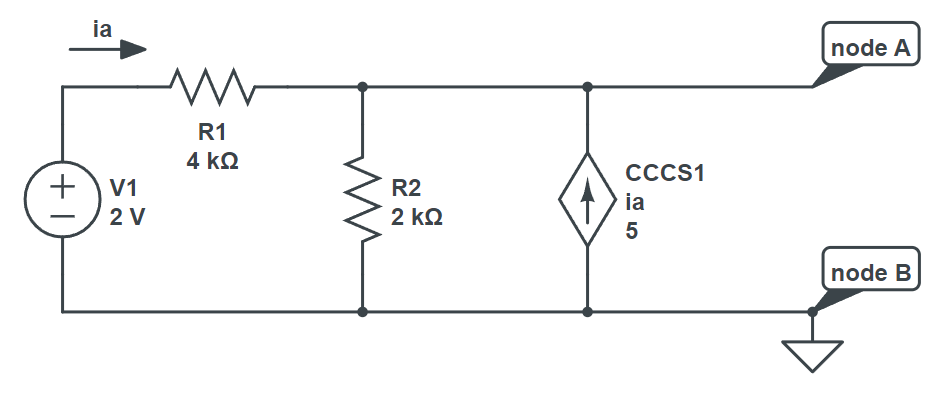
\includegraphics[scale=0.7]{circuit-1-2.png}
        \caption { Electric circuit with terminals A-B}
    \end{center}
\end{figure}

Using CircuitLab, we first measure the voltage at node A to obtain $v_{oc} = \SI{1.5}{V}$. We then attach a wire across terminals A-B to obtain $i_{sc} = \SI{3}{mA}$. We can then calculate $R_{th}$ such that

\begin{equation}
    \begin{split}
        R_{th} = \frac{V_{oc}}{i_{sc}} = \frac{\SI{1.5}{V}}{\SI{3}{mA}} = \SI{500}{\ohm}
    \end{split}
\end{equation}

From this, we build Thévenin's Circuit such that

\begin{figure}[H]
    \begin{center}
        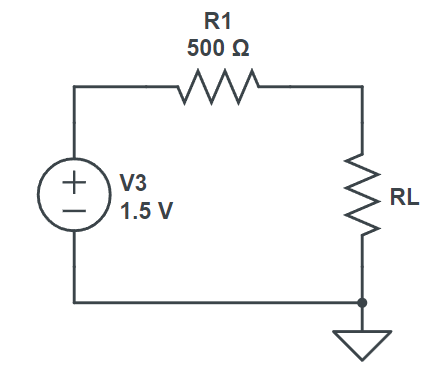
\includegraphics[scale=0.7]{circuit-2.png}
        \caption { Thévenin's Circuit with load resistor $R_L$}
    \end{center}
\end{figure}

To validate Thévenin's Theorem, we test various resistances across $R_L$ and compare them to the values obtained in Table (1) using the original circuit shown in Figure (1). 

\pagebreak

For example, testing $R_L = 56\Omega$ for Thévenin's circuit, we can use Ohm's Law to get that

\begin{equation}
    \begin{split}
        i_{s} &= \frac{v_{oc}}{R_{eq}} = \frac{1.5}{500 + 56} = \SI{2.6978}{mA} \\
        v_{L} &= \left(\frac{R_L}{R_L + 500}\right)v_{oc} = \left(\frac{56}{56 + 500}\right)(1.5) = \SI{151.079}{mV}
    \end{split}
\end{equation}

From Table (1) for $R_L = 56\Omega$, we see that Thévenin's equivalent circuit produces the same electrical quantities as the original circuit which proves Thévenin's Theorem experimentally. One interesting difference would be that the current through the voltage source would act differently than the current through the voltage source in the original circuit. This is because as $R_L$ becomes very large, and begins to act like an open circuit, no current would flow in Thévenin's circuit. However, in the original circuit, there are other branches for the current to flow through, thus current never approaches zero. In any case, this does not affect the validity of Thévenin's theorem. We can conclude that the graphs and data across the resistor $R_L$ obtained from the original circuit would apply to Thévenin's circuit load $R_L$. Lastly, in analyzing the power data and graph, we note that when $R_L = 500\Omega$, the power is at a maximum which is the same as $R_{th}$ as calculated in Equation (2). This proves the maximum power transfer theorem, which states that the power across the resistor $R_L$ is at a maximum when $R_L = R_{th}$. Thus, the experimental data agrees with theory.

\section{Conclusion}
From this lab, we gain a better understanding of the behavior of various electrical quantities across a resistor as the resistance changes. Furthermore, we confirm that values obtained from software are within a very small percent error with respect to the theoretical values which indicates that the software is sufficiently accurate. Additionally, we confirm the validity of Thévenin's Theorem by comparing the values produced by the original circuit and Thévenin's equivalent circuit.

\pagebreak

\section{CircuitLab Reference}
Below are the links to the circuits created for this lab in CircuitLab.

\begin{itemize}
    \item Original Circuit: \url{https://www.circuitlab.com/editor/#?id=gsme39a23q99}
    \item Thévenin's Circuit: \url{https://www.circuitlab.com/editor/#?id=z6wa4dha4een}
  \end{itemize}

\end{document}